\documentclass[10pt,twocolumn,letterpaper]{article}

\usepackage{cvpr}
\usepackage{times}
\usepackage{epsfig}
\usepackage{graphicx}
\usepackage{amsmath}
\usepackage{amssymb}
\usepackage{cite}
\usepackage{subcaption}
% Include other packages here, before hyperref.

% If you comment hyperref and then uncomment it, you should delete
% egpaper.aux before re-running latex.  (Or just hit 'q' on the first latex
% run, let it finish, and you should be clear).
\usepackage[breaklinks=true,bookmarks=false]{hyperref}

\cvprfinalcopy % *** Uncomment this line for the final submission

\def\cvprPaperID{****} % *** Enter the CVPR Paper ID here
\def\httilde{\mbox{\tt\raisebox{-.5ex}{\symbol{126}}}}

% Pages are numbered in submission mode, and unnumbered in camera-ready
%\ifcvprfinal\pagestyle{empty}\fi

\begin{document}

%%%%%%%%% TITLE
\title{Tracking-Learning-Detection Framework}

\author{Jasper Lin\\
Stanford University\\
Stanford, CA \\
{\tt\small jasperlin@stanford.edu}}
\maketitle
%\thispagestyle{empty}

%%%%%%%%% ABSTRACT

%%%%%%%%% BODY TEXT
\section{Introduction}
Object tracking is becoming an increasingly popular subfield within computer vision.  The increase in computing power and availability of high quality videos has resulted in a need for object tracking algorithms \cite{survey}. Tracking can be simply thought of as estimating the trajectory of objects within a series of image sequences. Difficulties arise in the form image noise, complex object motion,, nonrigid objects, illumination changes, and real time processing needs. The big difference between tracking algorithms is how they approach object representation, image feature selection, and how should the motion be modeled. Objects can be defined in many unique ways, including as points, shapes, silhouette, and skeletal models. Features can be represented as probabilities densities, templates, and appearance model. In general, it's important to choose the correct algorithm and representation that accurately fits the application. 

\subsection{Visual Tracking with Online Multiple Instance Learning}
	Babenko et. al developed an adaptive appearance model that tracked objects using detections \cite{MIL}. Their work focuses on how to choose positive and negative examples when updating an adaptive appearance model. Negative examples were usually drawn from the neighborhood of the tracker location. However, if the location of the tracker is wrong, this results in a suboptimal model that tends to drift with time. Because of this challenge, they implemented Multiple Instance Learning (MIL) for objection detection. In MIL, bounding box candidates can be stored in bags and labels are provided for the bag, not the individual instance. By bootstrapping itself, they allow for the learning algorithm to dictate the decision boundary for itself.

\subsection{Struck: Structured Output Tracking with Kernels}
Hare et. al also work on improving the adaptive tracking-by-detection model.  \cite{kernel} It has been shown that the use of support vector machines (SVMs) outperform boosting due to their generalization ability, robustness to label noise, and flexibility and object representation with kernels. The main contribution of the paper was creating a structured output tracking framework that allows us to skip the intermediate classification of samples in normal adaptive detection models. Instead of learning a classifier, the algorithm tries to predict different transformations that can occur. The use of kernels allows for easy representation of a variety of image features and can be combined together.

\section{Tracking-Learning-Detection Framework}
Kalal et. al develop the novel Tracking-Learning-Detection (TLD) framework that allows long-term tracking to be broken down into these three separate components \cite{tld}. The tracker follows the object from frame to frame. The detector localizes the appearances that have observed so far and corrects the tracker if necessary. The learning estimates the detector's errors and updates it to avoid further errors.
\subsection{Tracker}
The tracking component of TLD is based on Median-Flow tracker extended with failure detection. The tracker estimates the motion of the object between consecutive frames. It assumes the visibility of the object all times and fails if the objects is fully occluded or moves out of the object's view. In the original TLD framework, they choose to use the Lucas-Kanade tracker. 
\subsection{Object Detector Pipeline}
	The detector scans the original input image and creates all possible candidate bounding boxes at different scales and shifts. From these bounding boxes (~50k), the detector must decide whether the object is there or not. The object model M is a collection of positive and negatives patches, $M =\{p_1^+,p_2^+, ..., p_m^+, p_1^-,p_2^-,...,p_n^-\}$, where $p^+$ and $p^-$ represent object and patches respectively. From these patches, we need to generate features of our choosing and train a classifier to separate out the positive data and the negative data. Kalal et. al implemented an ensemble classifier that use Fern comparisons as features. The ensemble consists of $n$ base classifiers which performs a certain number of Fern comparisons. The Fern comparisons are generated offline at random and stay fixed throughout the run time. Random pairs of indexes are selected to be compared and each comparison returns a 0 or 1 depending on which pixel has higher intensity. All of these measurements are concatenated into $x$. This binary representation can then be indexed to an array of posteriors $P_i(y|x)$ where $y \in \{0,1\}$.  Each base classifier maintains this distribution of probabilities. The probability is estimated as $P_i(y|x) = \frac{\#p}{\#p + \#n}$. The initial base posteriors are set to 0 and are updated if the ensemble classification differs from the nearest neighbor classification. The nearest compares the current patch with the object model using relative similarity. If any of the patches align with a similarity greater than 0.6, the patch is considered an object. 
\subsection{Learning}
\subsubsection {P-expert}
The P-expert's role is to find new appearances of the object and increase the generalization of the object detector. The P-expert tries to find reliable parts of the trajectory and add this new information to the object model. In every frame, the P-expert outputs a decision about the reliability of the current location. If the location is reliable, the P-expert generates positive data that update the object model and the ensemble classifier.
\subsubsection{N-expert}
The N-expert generates negative training data. The N-experts assumes that the object can only occupy one location in the image. Thus, all areas surrounding the object are considered viable negative candidates. The N-expert is applied at the same time as the P-expert, so only if the trajectory is reliable. Patches that are far from the current bounding box are selected and can be used the update the object detector and classifier.
\section{My implementation}
I decided to follow the original implementation as closely as possible and mostly extend the project through examining and tuning some of the hyper parameters used in the paper. The biggest changes I made were to the object detector pipeline. When the detector searches for possible bounding boxes, I use the bounding box determined in previous frames to help limit the number of patches I am looking at. I calculate the movement of the center of the bounding box and estimate the trajectory and location of the bounding box in the current image. I threshold the candidate bounding boxes that are within a certain distance from the estimate trajectory. In addition, we can safely assume that the size of the object will not change significantly between frames so we can limit the bounding boxes we search for to those that have a certain range in size. To account for objects that might move out of the frame and lose the bounding box and then come back in, I assumed that these objects would reappear in the same area as they had originally left. So I keep track on the last existing bounding box and use that as the start of my search for bounding boxes. These limitations of search space significantly sped up the runtime. Another departure I made from the original paper was no longer filtering by the variance of the patches. I found that, while there is some sacrifice in runtime, the detector is generally more able to find objects in low light situations. In addition, I implemented Local Binary Pattern (LBP) as an alternative for converting patches to features.
\section{Code README}
The parameters for the fern classifier, number of classifiers and number of comparisons each, can be changed in $run\_TLD\_on\_video.m$. Limitations on the bounding box grid based on location and size is done in $tldDetection.m$. 
\section{Results and Discussion}
I implemented the TLD algorithm in MATLAB 2014B with 2.7 GHz Intel i5 processor and 8 GB of RAM. The tracking results using 10 classifiers each with 13 comparisons, like the original paper, for the 9 sets of images are shown in Table \ref{table:results1}.
\begin{table}
\begin{center}
\begin{tabular} {|c|c|c|c|c|}
\hline
&Average Overlap& Success Auc & mAP &Sec/Frame \\ \hline
Car4 & 0.796 & 0.796 & 0.941 & 1.2935 \\ 
Dancer2 & 0.726 & 0.731 & 1 & 0.978 \\ 
Deer & 0.449 & 0.467 & 0.55 & 10.07 \\
Bolt2 & 0.013 & 0.062& 0.01 & 0.118 \\
Fish & 0.329 & 0.348 & 0.256 & 13.089 \\
Human8 & 0.268 & 0.297 & 0.085 & 0.603 \\
Jumping & 0.48 & 0.493 & 0.568 & 13.807 \\
Man & 0.625 & 0.627 & 0.848 & 1.196 \\
Vase & 0.508 & 0.504 & 0.291 & 1.1034 \\\hline
\end{tabular}
\caption{TLD results with 10 classifiers with 13 comparisons each}
\label{table:results1}
\end{center}
\end{table}
\subsection{General Intuition and Challenges}
The algorithm, in general, performed very well on the video sequences with good lighting and relatively little motion. Car4 and Dancer2 are two examples. Throughout the video sequence, the tracker and the detector were able to follow the object even if the object did change shape, like in Dancer2, as shown in Figure \ref{fig:dancer}. This is a good indicator that the learning portion of the algorithm is in fact working and generating positive examples that help the tracker.  I also found that the rough object trajectory and size limitations significantly reduced the run time of many videos. The video sequences that do take longer are indicating that the bounding box was lost somewhere and the algorithm is searching a larger set of bounding boxes to find a potential match for the features.  \\
\begin{figure}
\begin{centering}
\begin{subfigure}[b]{0.4\textwidth}
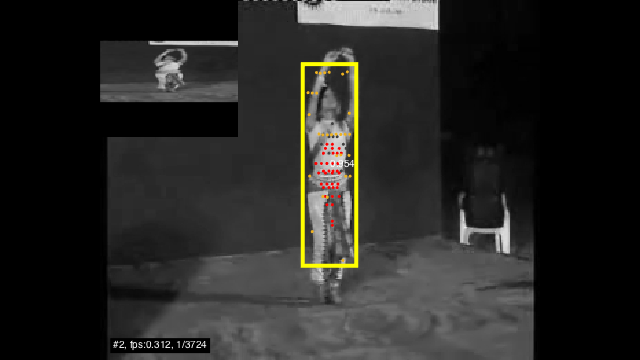
\includegraphics[width=\textwidth]{dancer1}
\end{subfigure}
\begin{subfigure}[b]{0.4\textwidth}
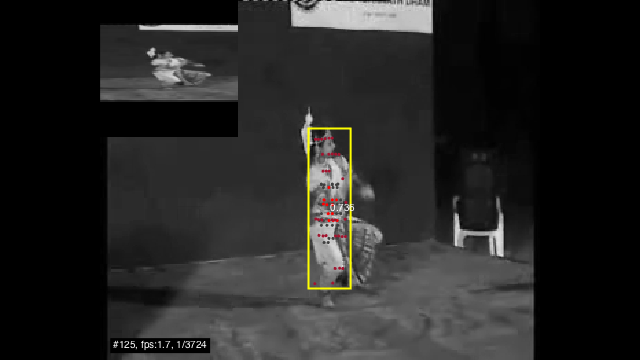
\includegraphics[width=\textwidth]{dancer3}
\end{subfigure}

\caption{TLD detecting different shapes of the object}
\label{fig:dancer}
\end{centering}
\end{figure}
Examples of video sequences that took longer but still seemed to perform in the end include the Deer and Jumping videos. These two videos are prime examples of videos that challenge the algorithm because of the presence of image blurriness. The motion of the object is greater than the frame-rate and blurs the image. This challenges the algorithm because the learned examples will not necessarily line up well with the current image, as shown in Figure \ref{fig:deer}. The bounding box is able to reinitialize when the image quality becomes better so it still manages to work throughout most of the video and only loses the box for several frames. \\
\begin{figure}
\begin{centering}
\begin{subfigure}[b]{0.4\textwidth}
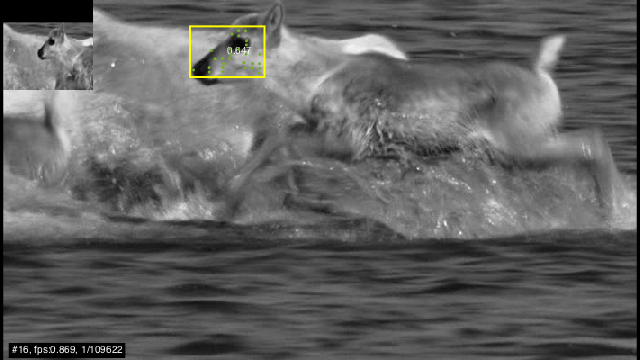
\includegraphics[width=\textwidth]{deer1}
\end{subfigure}
\begin{subfigure}[b]{0.4\textwidth}
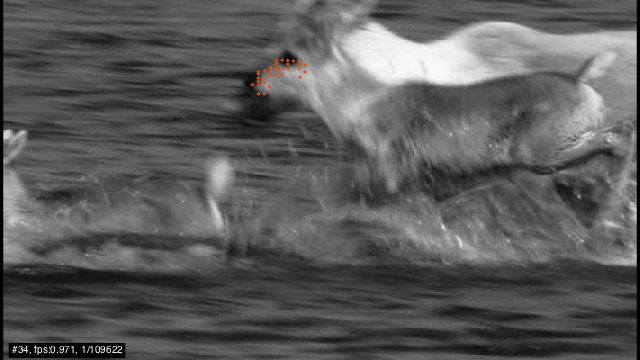
\includegraphics[width=\textwidth]{deer2}
\end{subfigure}
\caption{Image blurriness affecting tracking quality}
\label{fig:deer}
\end{centering}
\end{figure}
I purposely took out the variance threshold used in the original paper in hopes of allowing the algorithm bounding boxes under different lighting conditions. Compared to well-light images, darker images will tend to have lower variation in pixel intensity. By removing this step, I successfully track the person walking through the shadows in Human8, Figure \ref{fig:man} as well as never losing the person in Man. Unfortunately, in the example shown, the tracker seems to learn a lot of the shadows and loses the person as he walks back into the light. \\
\begin{figure}
\begin{centering}
\begin{subfigure}[b]{0.4\textwidth}
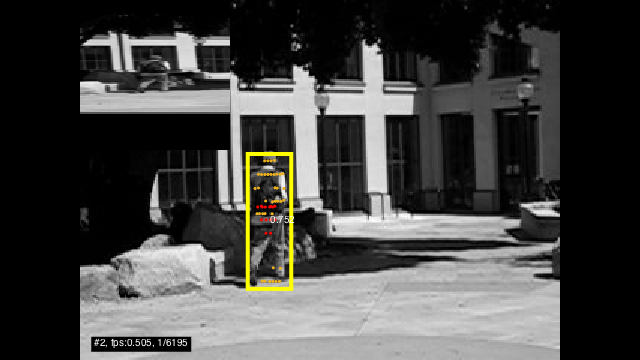
\includegraphics[width=\textwidth]{human1}
\end{subfigure}
\begin{subfigure}[b]{0.4\textwidth}
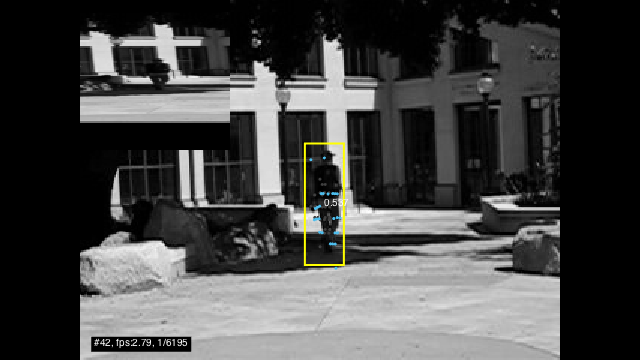
\includegraphics[width=\textwidth]{human2}
\end{subfigure}
\caption{Tracking through different lighting conditions}
\label{fig:man}
\end{centering}
\end{figure}
The sequence that my implementation struggled with the most was the Bolt2 video. The detector never really learns Bolt early on and the bounding box is lost within the first couple frames. One reason why the detector might struggle so much with the particular video is that the runners all look very similar. When we take negative samples from outside of the initial bounding box, we might train initial negative examples that prevent us from tracking Bolt. One possible solution is to implement a initial negative patterns that also checks the similarity of the sample bounding box with the ground truth before adding it to the dataset. 
\subsection{Varying Classifier Parameters}
In the original paper, they did not really discuss the motivation behind why they designed their classifier to have 10 base classifications and 13 comparisons. First, I kept the number of comparisons constant, 13, but varied the number of base classifiers. The results are shown in Figure \ref{fig:classifiers}. Surprisingly, there doesn't seem to be a consistent relationship between the number of classifiers used and the performance of the algorithm. One simple explanation could be that the video sequences chosen are fairly simple and there is no need for many classifiers. In the one video that does have significant amounts of rotation and movement, the Vase, the 30 classifiers outperformed the other runs by a large margin. \\
\begin{figure}
\begin{centering}
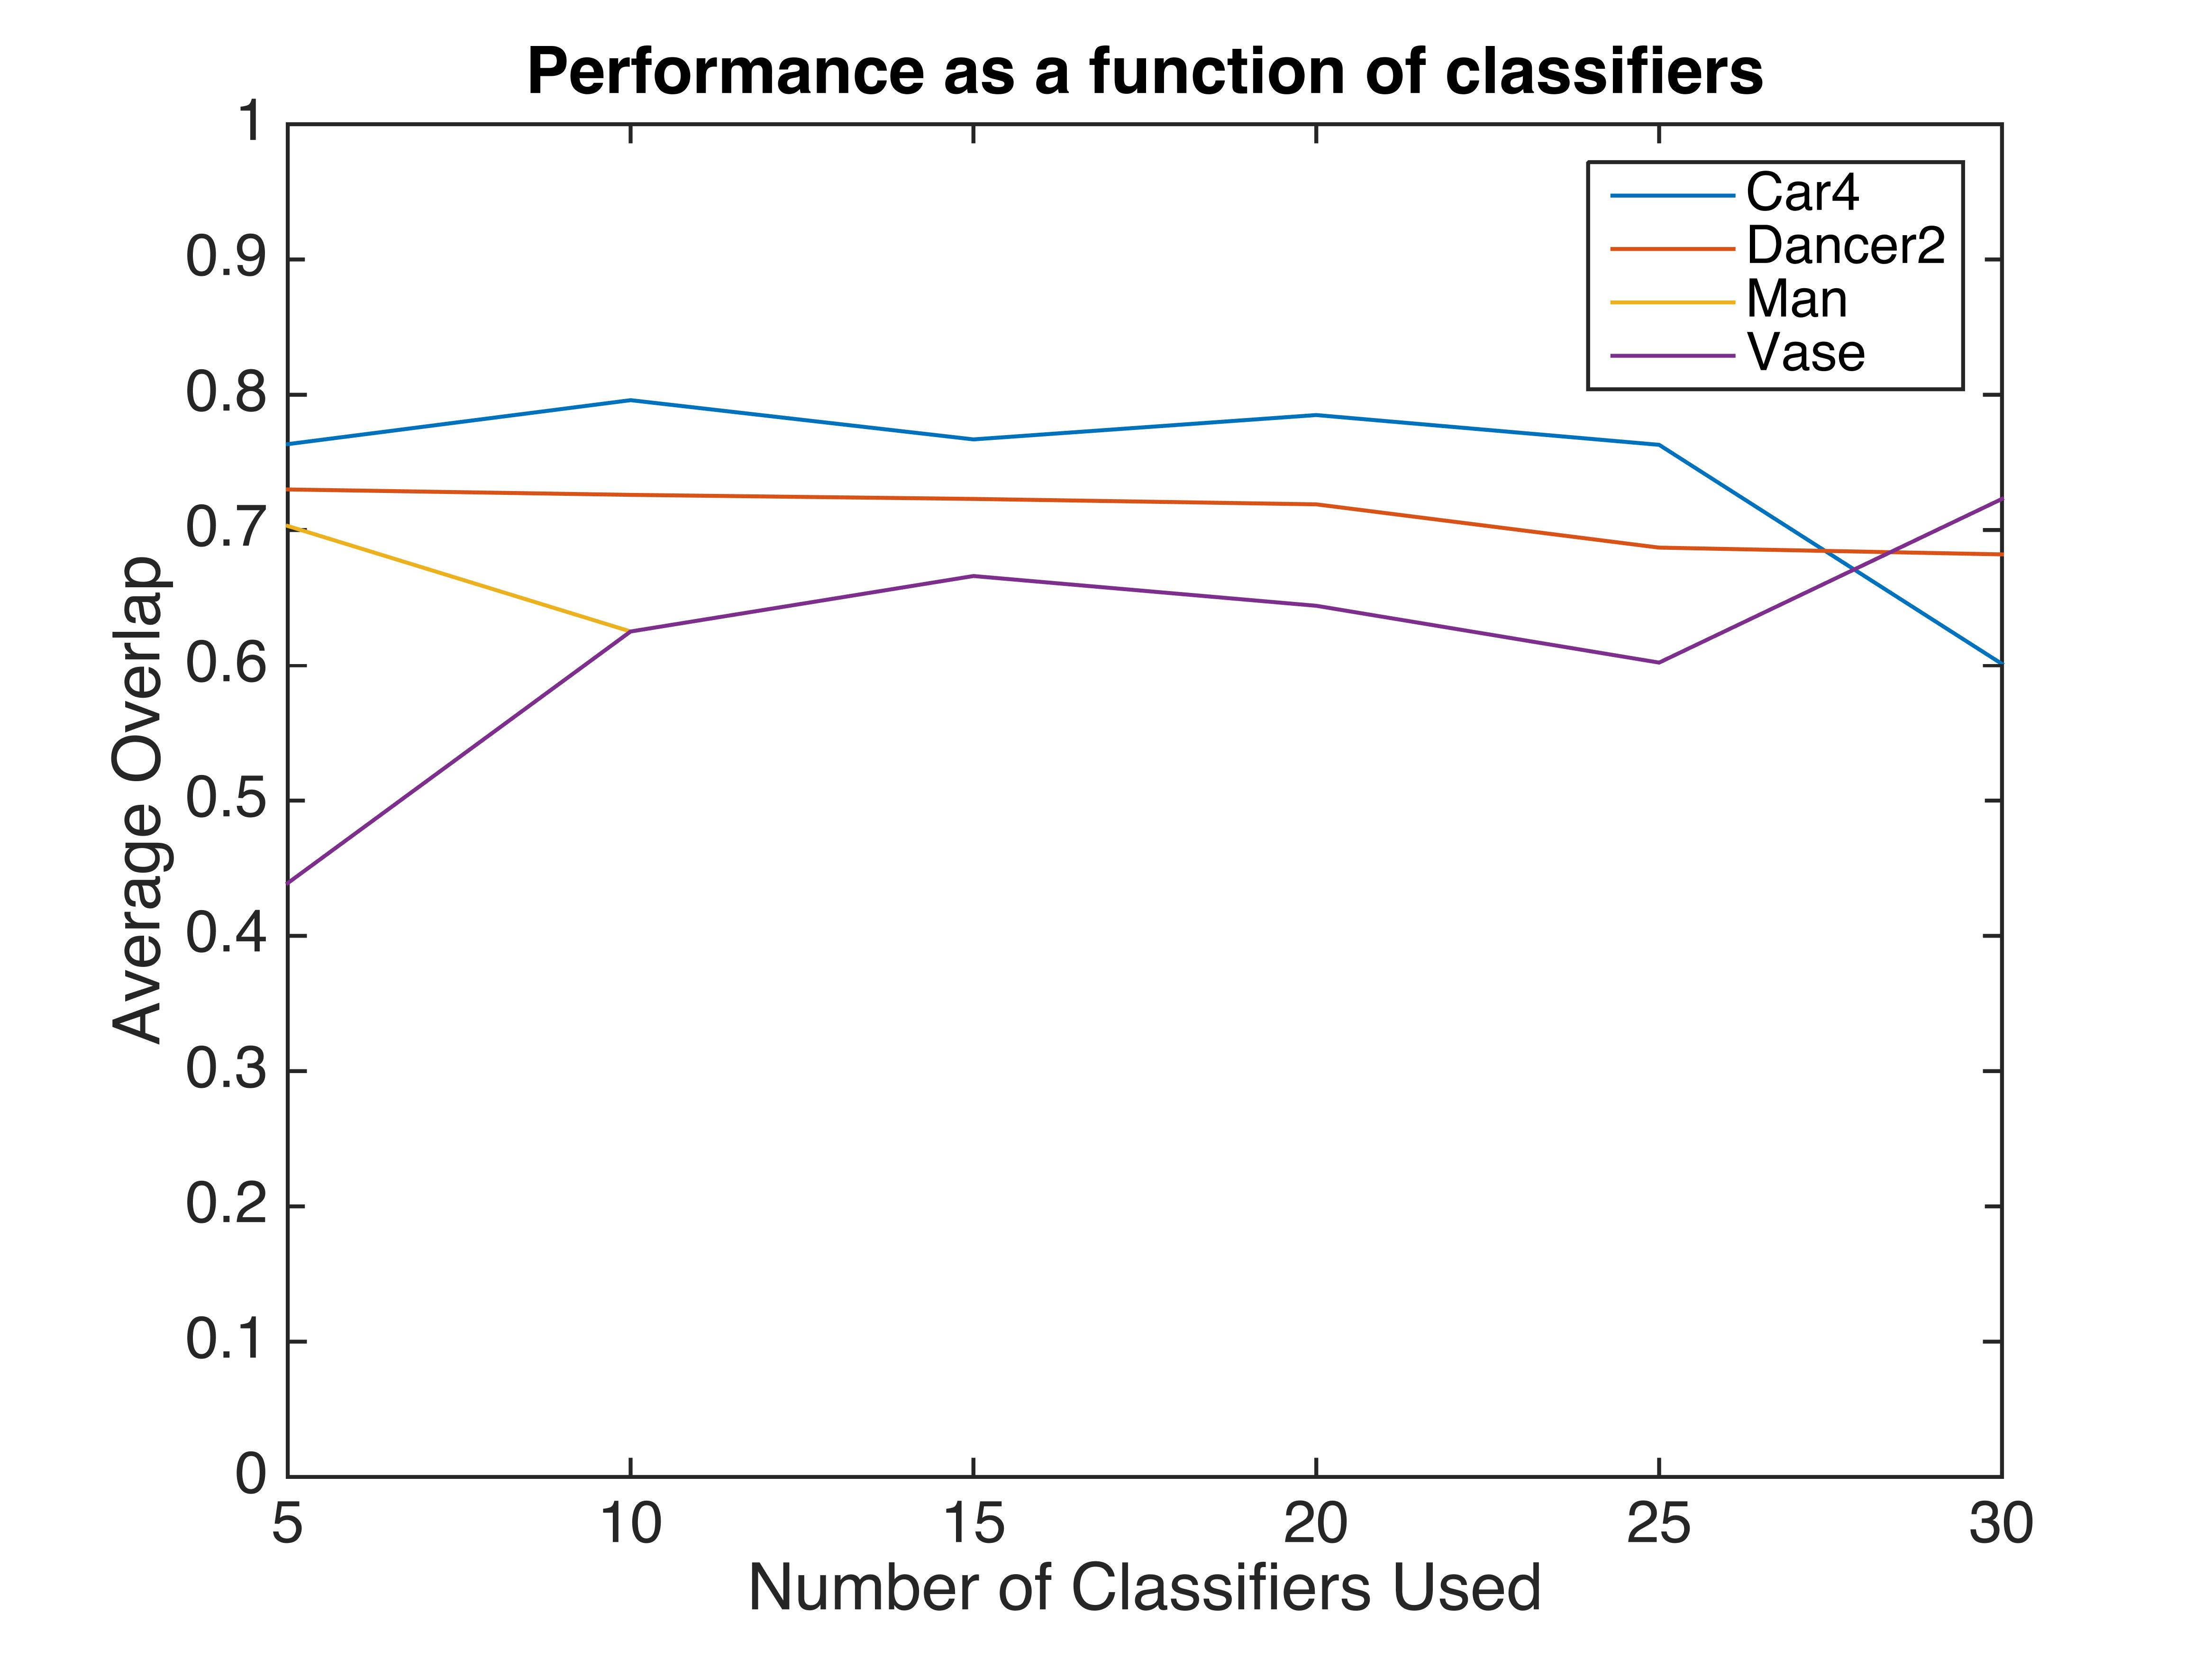
\includegraphics[width=0.4\textwidth]{classifiers}
\caption{Overlap as a function of number of classifiers used}
\label{fig:classifiers}
\end{centering}
\end{figure}
Next, I looked at keeping the number of base classifiers constant but changing the number of comparisons made. I initially thought that increasing the comparisons made would significantly reduce the accuracy of the results due to an exponentially more sparse posterior distribution. However, from some preliminary experiments, shown in Figure \ref{fig:comparisons}, the overlap accuracy seem to be best in the range of 10-15 comparisons. \\
\begin{figure}
\begin{centering}
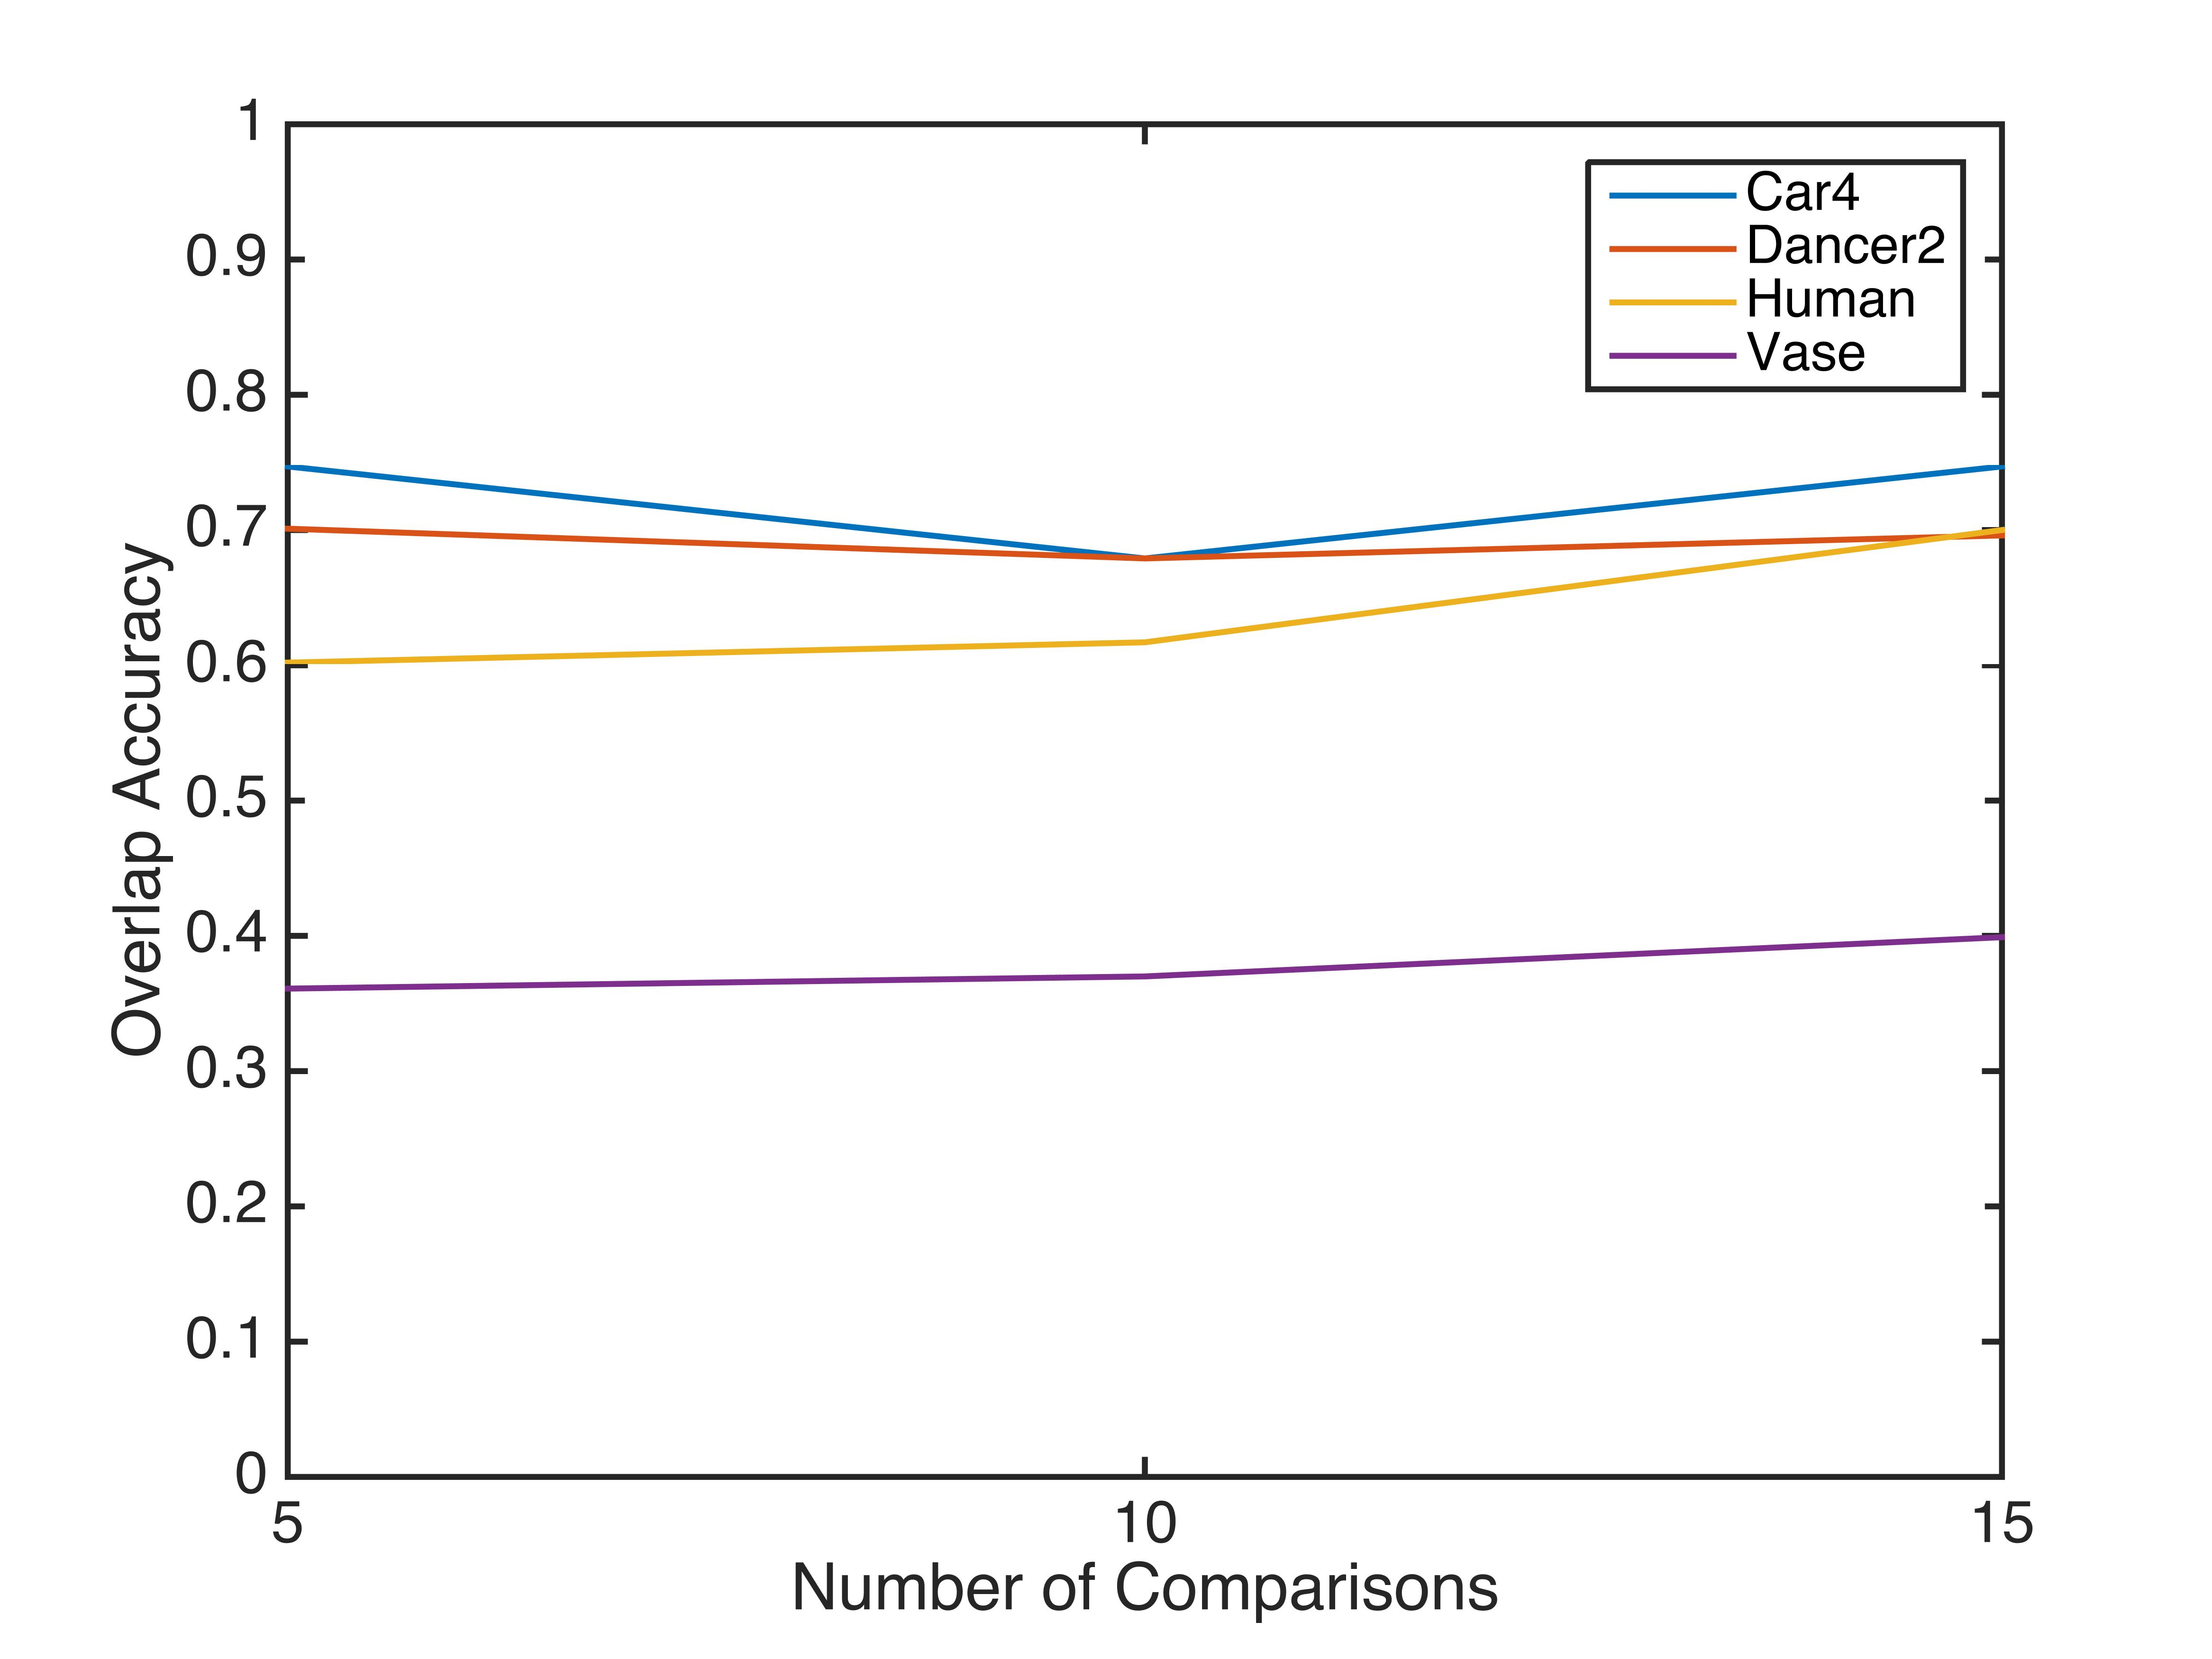
\includegraphics[width=0.4\textwidth]{comparisons}
\caption{Overlap as a function of number of comparisons used}
\label{fig:comparisons}
\end{centering}
\end{figure}
One note about both experiments. The algorithm did not necessarily take longer to run with increased number of classifiers/comparisons made. In many cases, it varied depending on the video. How often the learning process is called is what separates these different tests and each video will learn a different number of times based on how strong the confidences are.  
\subsection{Local Binary Pattern Experiments}
The results of using the LBP instead of just subtracting the mean of the resized image were surprisingly poor. Almost all image sequences lost the bounding box extremely early. I notice that the confidences outputted by the classifier were relatively low when using the LBP features. This then caused the P-expert have low confidence in the reliability of the bounding box and new features were almost never learned. Possible explanations for this include the greater sensitivity of a texture detector to light and pose. In addition, the resized patches of 25x25 were significantly smaller than the ground truth bounding boxes. The resizing may result in the loss of important texture information, causing the features to be extremely noisy.

\bibliography{egbib}
\bibliographystyle{ieee}
\nocite{*}

\end{document}
